\colorlet{mylightgray}{black!30}
\colorlet{mydarkgray}{black!50}


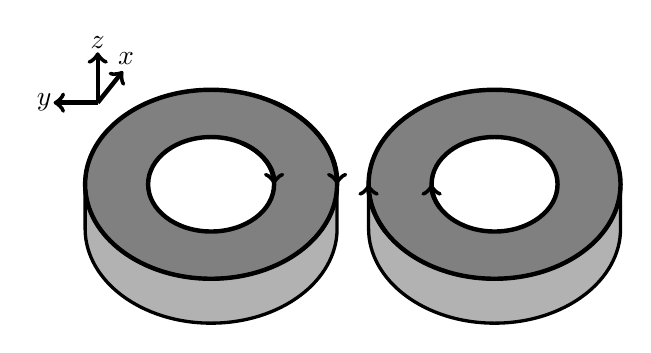
\begin{tikzpicture}[scale=0.4]
  \def\Rx{4.0}      % tank horizontal radius
  \def\Ry{3.0}      % tank vertical radius
  \def\rx{0.5*\Rx} % column horizontal radius
  \def\ry{0.5*\Ry} % column vertical radius
  \def\H{1.5}       % height tank
  \def\h{0.94*\H}   % height water
  \def\zob{9.0}   % height water

  \draw[very thick, fill=mylightgray] (-\Rx,\h) -- (-\Rx,0) arc (180:360:{\Rx} and {\Ry}) -- (\Rx,\h);
  \draw[very thick, fill=mylightgray] (\zob-\Rx,\h) -- (\zob-\Rx,0) arc (180:360:{\Rx} and {\Ry}) -- (\zob+\Rx,\h);

  \draw[fill=mydarkgray, very thick] (0,\h) ellipse ({\Rx} and {\Ry});
  \draw[fill=mydarkgray, very thick] (\zob,\h) ellipse ({\Rx} and {\Ry});

  \draw[ultra thick, fill=white] (0,\h) ellipse ({\rx} and {\ry});
  \draw[ultra thick] (0,\h) ellipse ({\Rx} and {\Ry});

  \draw[ultra thick, fill=white] (\zob,\h) ellipse ({\rx} and {\ry});
  \draw[ultra thick] (\zob,\h) ellipse ({\Rx} and {\Ry});

  \draw[<-, ultra thick] (0+\rx, \h) arc [start angle=0, end angle=60, x radius ={\rx}, y radius={\ry}];
  \draw[<-, ultra thick] (0+\Rx, \h) arc [start angle=0, end angle=60, x radius ={\Rx}, y radius={\Ry}];

  \draw[<-, ultra thick] (\zob-\rx, \h) arc [start angle=180, end angle=210, x radius ={\rx}, y radius={\ry}];
  \draw[<-, ultra thick] (\zob-\Rx, \h) arc [start angle=180, end angle=210, x radius ={\Rx}, y radius={\Ry}];

  \draw[ultra thick, ->] (-3.6, 4.0) -- (-2.8, 5.0);
  \node at (-2.7, 5.4) {$x$};
  \draw[ultra thick, ->] (-3.6, 4.0) -- (-5.0, 4.0);
  \node at (-5.3, 4.0) {$y$};
  \draw[ultra thick, ->] (-3.6, 4.0) -- (-3.6, 5.6);
  \node at (-3.6, 5.9) {$z$};


\end{tikzpicture}

